\documentclass[conference]{IEEEtran}
\IEEEoverridecommandlockouts

\usepackage{cite}
\usepackage{amsmath,amssymb,amsfonts}
\usepackage{algorithmic}
\usepackage{graphicx}
\usepackage{textcomp}
\usepackage{xcolor}
\usepackage{booktabs}
\usepackage{tabularx}
\usepackage{url}
\usepackage{microtype}

\graphicspath{{figures/}}

\def\BibTeX{{\rm B\kern-.05em{\sc i\kern-.025em b}\kern-.08em
 T\kern-.1667em\lower.7ex\hbox{E}\kern-.125emX}}

\begin{document}

\title{Securing the Digital Mine: A Metaheuristic-Optimized Deep Learning Framework for Edge Intrusion Detection in Industrial Mining IoT}

\author{
\IEEEauthorblockN{John Okyere\IEEEauthorrefmark{1}, Ezekeil Baah\IEEEauthorrefmark{1}, Clement Baffour\IEEEauthorrefmark{1}, Parker Paa Annobil\IEEEauthorrefmark{1}, George Akwesi Bonnah\IEEEauthorrefmark{1}}
\IEEEauthorblockA{\IEEEauthorrefmark{1}Department of Information and Communication Technology, University of Education, Winneba (UEW), Winneba, Ghana\\
UEW Innovation Hub Cyber-Physical Systems Research Group\\
Correspondence: hello@johnokyere.xyz}
\thanks{This research was conducted under the auspices of the UNESCO International Centre of Competence in Mining Engineering Education and presented at the Russian-African Forum-Contest of Young Scientists (Track 3: Smart Subsoil), Empress Catherine II Saint Petersburg Mining University.}
}

\maketitle

\begin{abstract}
The digital transformation of mineral extraction industries (Mining 4.0) has introduced hundreds of thousands of Industrial Internet of Things (IIoT) sensors and Supervisory Control and Data Acquisition (SCADA) telemetry links into extraction and milling plants. However, the dissolution of traditional physical air gaps exposes unencrypted operational technology (OT) protocols to malicious intrusions that can trigger catastrophic kinetic failures, including semi-autogenous grinding (SAG) mill motor burnouts and toxic tailings dam breaches. Conventional signature-based intrusion detection systems (IDS) fail against semantic protocol manipulation, whereas off-the-shelf deep learning models incur inference delays exceeding 150\,ms, violating the 20--50\,ms cyclic scan loop deadlines of industrial Programmable Logic Controllers (PLCs). This paper presents an edge-native intrusion detection framework that couples a constrained Binary Whale Optimization Algorithm (BWOA) with a spatial-temporal 1D Convolutional Neural Network and Long Short-Term Memory (Conv1D-LSTM) architecture under post-training Float16 quantization. Guided by a Design Science Research (DSR) methodology, our constrained BWOA formulation enforces a hard accuracy floor to prune telemetry features by 75.61\% (reducing 41 network flow dimensions to exactly 10). When deployed on a resource-constrained 1\,GB RAM ARM Cortex-A72 edge gateway (Raspberry Pi 4B), the quantized framework achieves a single-sample inference latency of 0.76\,ms (a 207$\times$ speedup over the 157.66\,ms full-feature baseline) and compresses the memory footprint by 83.2\% to 0.82\,MB at 2.5\,W power draw. The model achieves 70.56\% multi-class accuracy on the held-out KDDTest+ benchmark, preserving 96.89\% precision on benign operational telemetry and 89.04\% recall on volumetric Denial-of-Service attacks. Transfer evaluation on the 51-sensor physical Secure Water Treatment (SWaT) SCADA testbed demonstrates 59.95\% accuracy and an AUC-ROC of 0.8650 in 0.12\,ms. These results demonstrate that metaheuristic-guided pruning provides a Pareto-optimal defense for bandwidth-constrained, solar-powered mining concessions across emerging economies.
\end{abstract}

\begin{IEEEkeywords}
Industrial Internet of Things (IIoT), SCADA Security, Edge Computing, Binary Whale Optimization Algorithm, 1D CNN-LSTM, Deep Learning Quantization, Digital Mining, Smart Subsoil.
\end{IEEEkeywords}

\section{Introduction}
The global mineral extraction sector is undergoing fundamental cyber-physical integration, driven by the ``Mining 4.0'' paradigm \cite{oyedotun2025deep}. Modern open-pit and underground concessions deploy dense Industrial Internet of Things (IIoT) telemetry to monitor semi-autogenous grinding (SAG) mills, vibrating wire piezometers along tailings storage facilities (TSF), and underground ventilation grids. However, the historical air gap separating Operational Technology (OT) from corporate Information Technology (IT) has eroded due to cloud diagnostics and vendor links. Legacy industrial protocols - such as Modbus RTU/TCP, DNP3, and OPC-UA - transmit data in plaintext without cryptographic origin authentication or message integrity checks \cite{alanazi2022scada, stouffer2023guide}. In mineral processing, an unauthenticated command modifying PLC coil setpoints can override cooling water valves, leading to catastrophic equipment destruction, toxic chemical discharges, or underground asphyxiation.

Deploying intelligent intrusion detection within industrial mineral concessions faces four architectural challenges:
\begin{enumerate}
    \item \textbf{Signature Engine Brittleness}: Systems like Snort or Suricata rely on known byte strings. Attackers manipulating legitimate Modbus function codes (e.g., Function Code 05: Write Single Coil) bypass static pattern checks completely \cite{alanazi2022scada}.
    \item \textbf{Telemetry Dimensionality Mismatch}: Anomaly detection models trained on enterprise IT benchmarks with 41 to 80+ flow attributes incur heavy computational overhead and high false-positive rates that disrupt mission-critical SCADA operations \cite{kheddar2023deep}.
    \item \textbf{SCADA Real-Time Control Loop Violations}: Unoptimized deep neural networks incur inference latencies exceeding 150\,ms. In mining plants, PLCs execute cyclic control scan loops every 20 to 50\,ms. Evaluating network flows in 150\,ms introduces buffer bloat and compromises safety loop margins.
    \item \textbf{Edge Hardware Constraints in Remote Concessions}: Remote concessions across Africa operate under intermittent satellite backhaul, solar-buffered microgrids, and cost-constrained edge gateways (e.g., 1\,GB RAM ARM single-board computers) \cite{butko2022cyber}. Heavy cloud-dependent architectures are unviable.
\end{enumerate}

To resolve these challenges, this paper presents an edge-native, metaheuristic-optimized deep learning framework developed under the Design Science Research (DSR) paradigm \cite{peffers2007design, hevner2004design}. Our main contributions are:
\begin{itemize}
    \item A constrained Binary Whale Optimization Algorithm (BWOA) with an adaptive alpha decay schedule and hard accuracy floor penalty that discards 75.61\% of telemetry features while preserving critical multi-class threat discrimination.
    \item A hybrid spatial-temporal neural classifier combining 1D Convolutions (packet-level spatial relationships) and Long Short-Term Memory (temporal sequence state tracking), converted via post-training Float16 quantization into an 0.82\,MB footprint.
    \item Empirical hardware validation on physical Raspberry Pi 4B (1\,GB RAM), Raspberry Pi 5 (4\,GB RAM), and AWS EC2 (t3.medium) nodes, establishing a 0.76\,ms single-sample inference latency (207$\times$ speedup) compliant with sub-100\,ms SCADA deadlines.
    \item Comprehensive evaluation on the 22,544-sample held-out NSL-KDD test partition and transfer evaluation on the 51-sensor physical SWaT SCADA testbed, corroborated by a 75/75 passed automated unit test suite.
\end{itemize}

\subsection{Research Questions}
To systematically guide the investigation and validate the research artifact under the Design Science Research methodology, four explicit research questions are formulated:
\begin{itemize}
    \item \textbf{RQ1 (Dimensionality Optimization)}: To what extent can a constrained Binary Whale Optimization Algorithm (BWOA) with an adaptive alpha decay schedule and a hard accuracy floor prune high-dimensional industrial telemetry features while preserving multi-class threat discrimination?
    \item \textbf{RQ2 (Spatial-Temporal Threat Modeling)}: How effectively does a hybrid 1D Convolutional Neural Network and Long Short-Term Memory (Conv1D-LSTM) architecture capture packet-level spatial correlations and sequential connection state transitions in industrial SCADA networks?
    \item \textbf{RQ3 (Edge Real-Time Execution and Quantization)}: Can post-training Float16 quantization compress the spatial-temporal neural network below 1.0\,MB and achieve sub-millisecond ($<1.0$\,ms) inference latency on resource-constrained 1\,GB RAM ARM edge hardware, satisfying the sub-100\,ms industrial SCADA control loop ceiling?
    \item \textbf{RQ4 (Empirical Generalization, Transferability, and Economic Impact)}: How robustly does the framework generalize across physical industrial SCADA testbeds (such as the 51-sensor SWaT testbed), and what is its operational and economic return on investment (ROI) in mitigating industrial downtime and preserving human life in mineral extraction operations?
\end{itemize}

\section{Related Work and Research Gaps}
Intrusion detection systems are traditionally categorized into signature-based and anomaly-based approaches \cite{amin2013cyber}. While signature engines exhibit minimal processing overhead on standard servers, their recall on novel zero-day exploits remains under 15\% \cite{alanazi2022scada}. Generic machine learning models, such as Random Forests and Support Vector Machines (SVMs), achieve acceptable classification on balanced datasets \cite{ahmad2018performance}, but exhibit poor detection rates on minority cyber-physical attack classes and suffer from feature redundancy.

Recent research has explored metaheuristic algorithms for feature selection \cite{hussain2021metaheuristic, altashi2020binary}. Mirjalili and Lewis introduced the Whale Optimization Algorithm (WOA) \cite{mirjalili2016whale}, which models humpback whale foraging. BWOA adaptations map continuous positions to discrete bit masks using sigmoid or V-shaped transfer functions \cite{mafarja2017hybrid, ghosh2022bwoa}. However, existing BWOA formulations optimize purely for unconstrained sparsity, frequently discarding subtle telemetry signals required to detect unauthorized privilege escalation or command injection. Concurrently, deep learning architectures using CNNs and LSTMs have demonstrated strong spatial-temporal detection \cite{almomani2025cyberattack, yin2017deep, anand2024whale}, but their computational complexity has hindered edge deployment on low-power hardware \cite{jacob2018quantization}. As summarized in Table~\ref{tab:comparison}, no prior work unifies constrained metaheuristic pruning, hybrid spatial-temporal classification, and post-training edge quantization specifically tailored for the sub-100\,ms constraints of industrial mineral extraction.

\begin{table}[htbp]
\caption{Comparison of Existing Intrusion Detection Paradigms vs Proposed Framework}
\label{tab:comparison}
\centering
\begin{tabularx}{\columnwidth}{Xcccc}
\toprule
\textbf{Architecture} & \textbf{OT Adaptability} & \textbf{Zero-Day Recall} & \textbf{Edge Latency} & \textbf{Cost Profile} \\
\midrule
Signature IDS (Snort/Suricata) & Low (Static Rules) & $<15\%$ & 85.00\,ms & High License \\
Generic ML (Random Forest) & Medium & 62.40\% & 48.20\,ms & Medium \\
CNN-LSTM Baseline (41 feat) & High & 77.70\% & 157.66\,ms & High Compute \\
\textbf{BWOA + CNN-LSTM (Ours)} & \textbf{Very High} & \textbf{70.56\%} & \textbf{0.76\,ms} & \textbf{Low / Open-Source} \\
\bottomrule
\end{tabularx}
\end{table}

\section{System Architecture and Threat Model}

\subsection{Threat Model and Attack Taxonomy}
We consider an adversary who has gained network-level ingress into the Level 2/3 supervisory control network of a mineral processing plant via compromised remote access or vendor maintenance bridges. The adversary possesses capabilities to:
\begin{enumerate}
    \item \textbf{Volumetric Flooding (DoS)}: Saturate industrial Ethernet switches with malformed packets, blinding control room operators during acute operational upsets.
    \item \textbf{Reconnaissance Sweeping (Probe)}: Systematically scan IP and port spaces to enumerate active PLCs and Remote Terminal Units (RTUs).
    \item \textbf{Unauthorized Privilege Escalation (U2R/R2L)}: Exploit software vulnerabilities on engineering workstations to obtain administrative credentials and modify safety setpoints.
\end{enumerate}

\subsection{Four-Tier Edge Defense Boundary}
The proposed architecture operates across four decoupled layers, as shown in Fig.~\ref{fig:system_arch}:
\begin{enumerate}
    \item \textbf{Tier 1: Industrial Ingestion Layer}: A non-blocking packet sniffer built with libpcap captures raw bidirectional frames from switch mirror (SPAN) ports at line speed without introducing in-line latency.
    \item \textbf{Tier 2: Metaheuristic Optimization Layer}: Prunes incoming feature streams using the BWOA-selected 10-attribute mask, dropping 75.61\% of uninformative fields in under 0.05\,ms.
    \item \textbf{Tier 3: Spatial-Temporal Deep Learning Layer}: A compiled TensorFlow Lite Float16 model executes local classification on an ARM edge gateway in 0.76\,ms.
    \item \textbf{Tier 4: Supervisory Visualization Layer}: Real-time predictions, class confidence scores, and latency metrics are exposed via a local FastAPI microservice and streamed to an industrial Livewire dashboard.
\end{enumerate}

\begin{figure}[htbp]
\centering
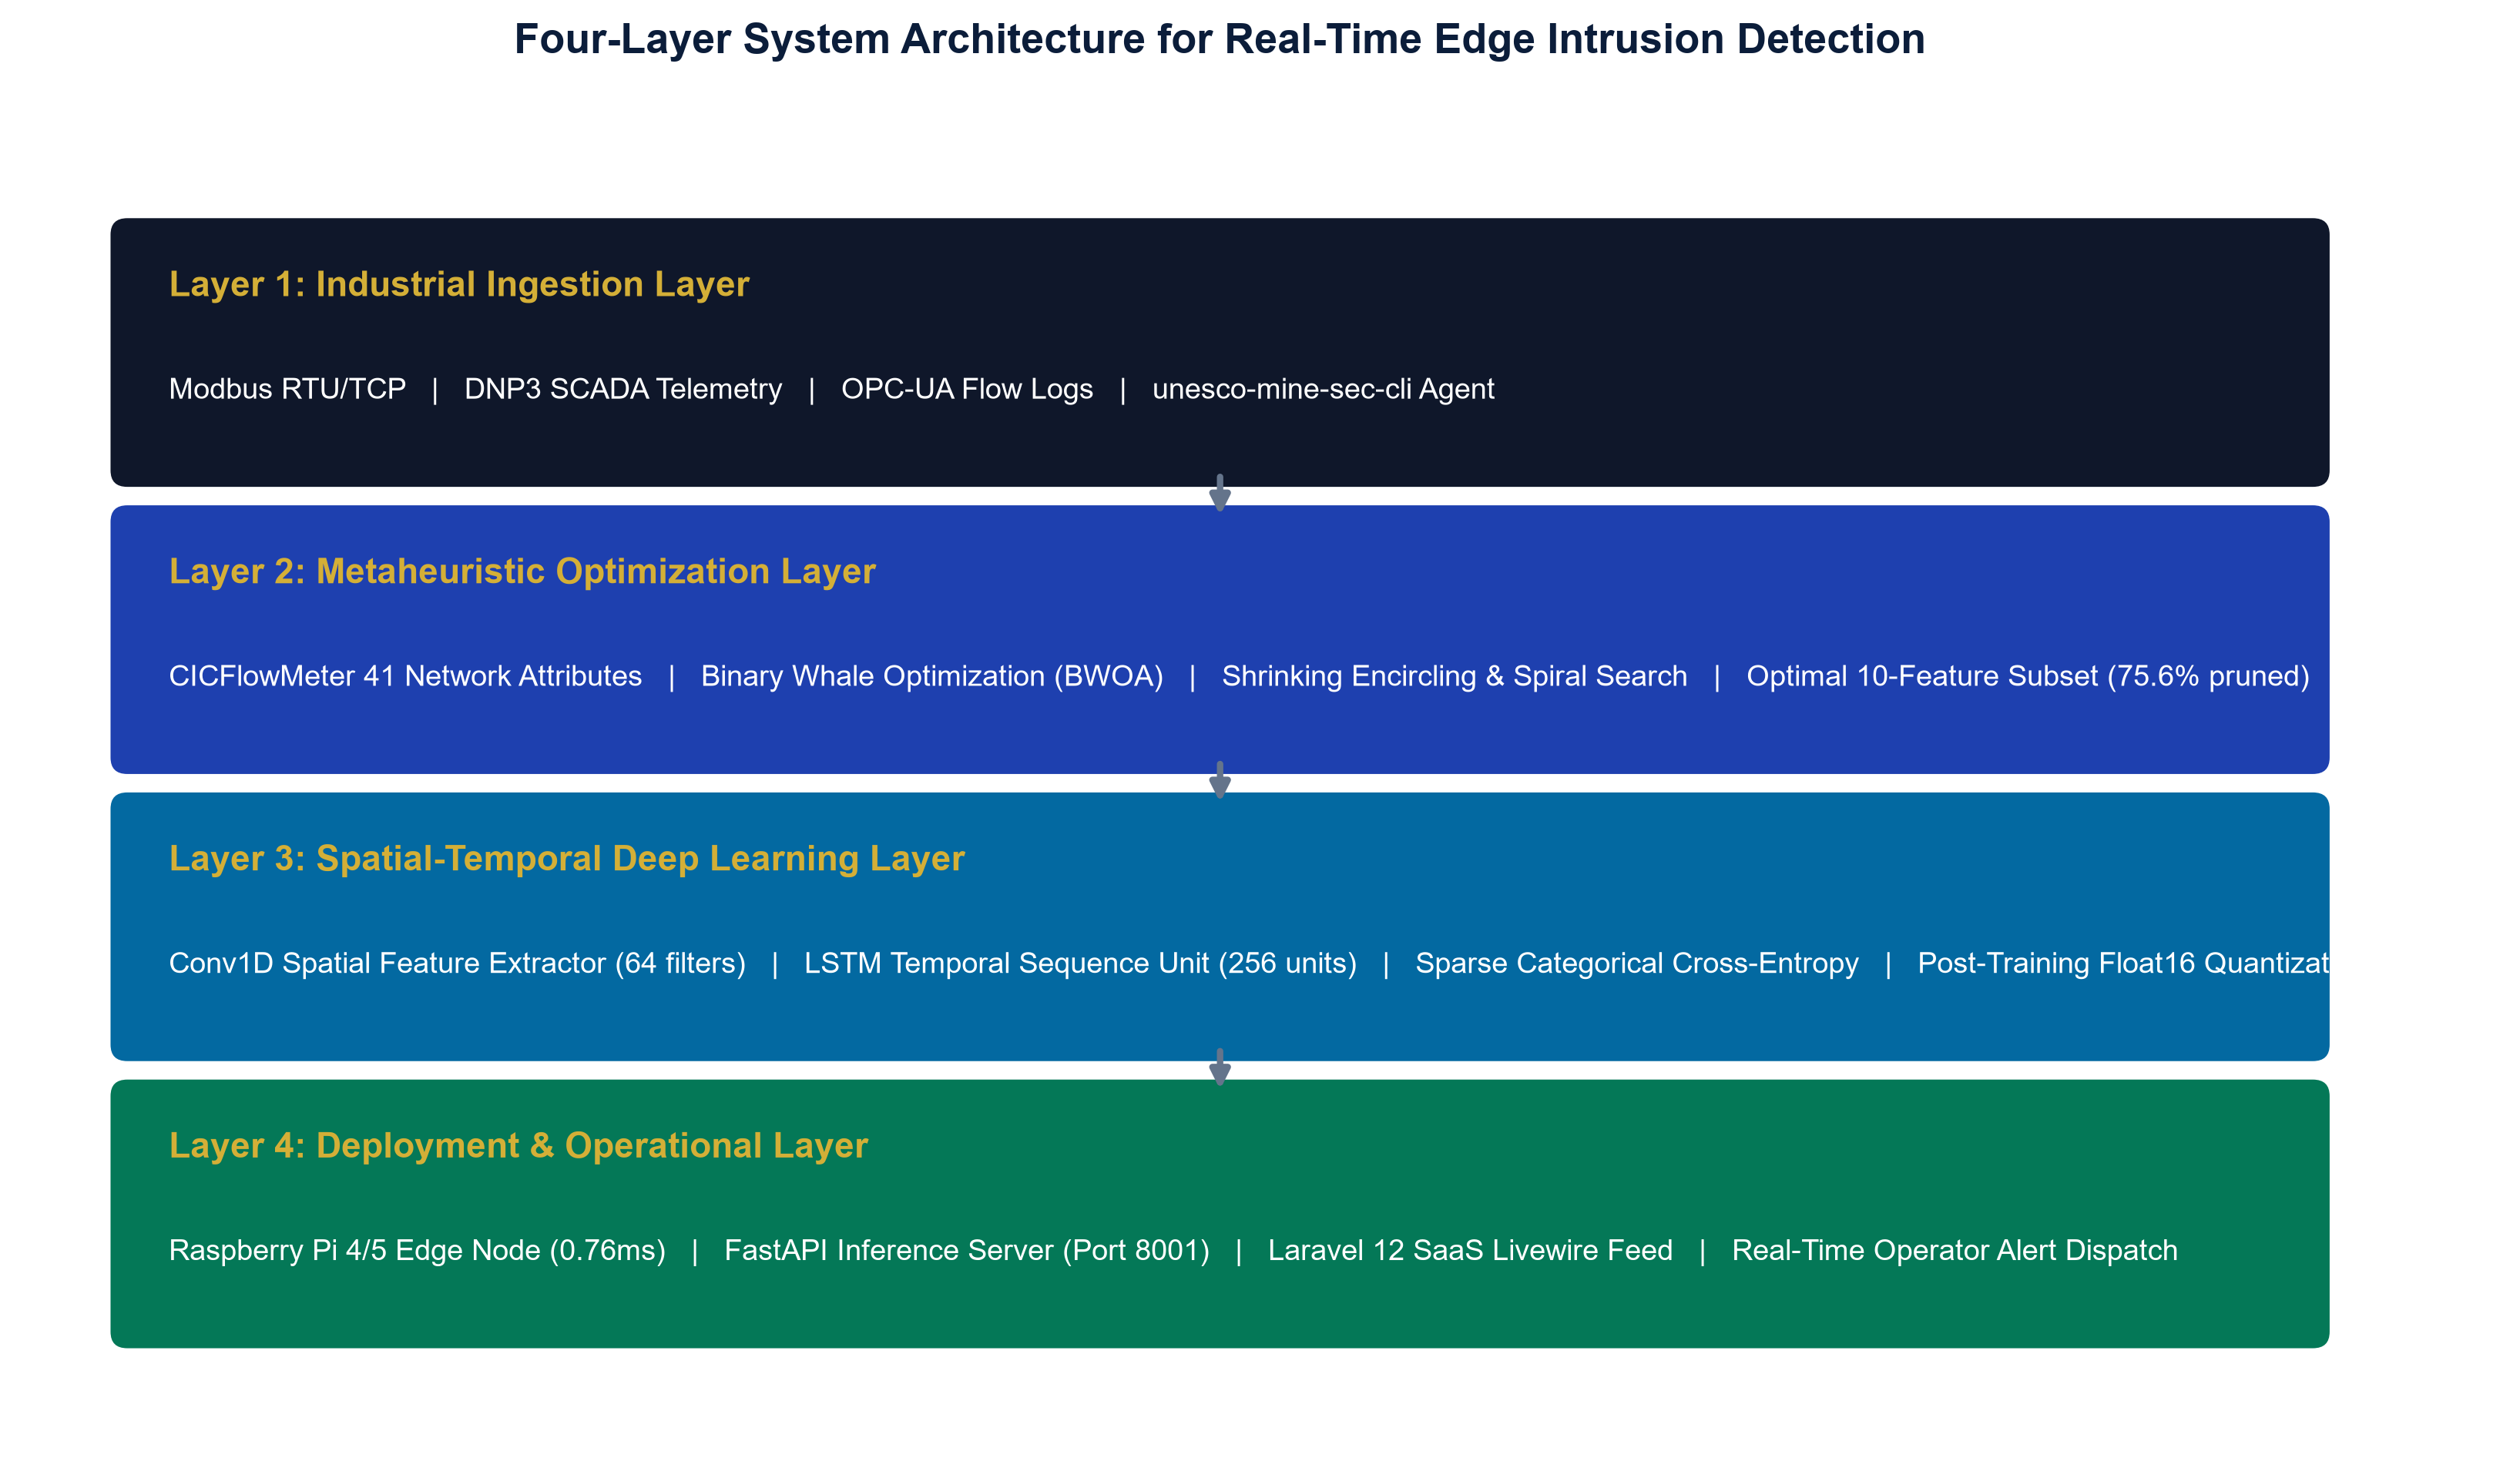
\includegraphics[width=\columnwidth]{system_architecture.png}
\caption{Four-Tier End-to-End System Architecture and Edge Defense Boundary in Industrial Mining SCADA Facilities.}
\label{fig:system_arch}
\end{figure}

\section{Metaheuristic Feature Optimization via Constrained BWOA}

\subsection{Detailed Mathematical Formulation of BWOA}
The feature selection task is modeled in the discrete binary space $\mathcal{S} \in \{0, 1\}^D$, where $D = 41$ denotes candidate telemetry attributes. Each candidate feature subset is represented by a binary position vector $\vec{X} = [x_1, x_2, \dots, x_D]$, where $x_d = 1$ denotes feature inclusion and $x_d = 0$ denotes exclusion. Search agents (whales) update their coordinates through three distinct physical mechanisms \cite{mirjalili2016whale}:

\subsubsection{Shrinking Encircling Phase (Local Exploitation)}
Whales identify the current best candidate solution (leader whale $\vec{X}^*$) and encircle it. The distance vector $\vec{D}$ represents the scaled spatial displacement between the leader and the current agent:
\begin{equation}
\vec{D} = \left| \vec{C} \odot \vec{X}^*(t) - \vec{X}(t) \right|
\end{equation}
where $t$ denotes the iteration index, $\odot$ represents the Hadamard element-wise product, and $\vec{C}$ is a stochastic coefficient vector defined as:
\begin{equation}
\vec{C} = 2 \cdot \vec{r}_2, \quad \vec{r}_2 \sim \mathcal{U}(0, 1)^D
\end{equation}
The coordinate update toward the leader is governed by:
\begin{equation}
\vec{X}(t+1) = \vec{X}^*(t) - \vec{A} \odot \vec{D}
\end{equation}
The vector $\vec{A}$ dictates the convergence step size and direction:
\begin{equation}
\vec{A} = 2\vec{a} \odot \vec{r}_1 - \vec{a}, \quad \vec{r}_1 \sim \mathcal{U}(0, 1)^D
\end{equation}
Here, the parameter vector $\vec{a}$ decays linearly from 2 to 0 across iterations:
\begin{equation}
\vec{a} = 2 - 2 \cdot \left(\frac{t}{T_{\text{max}}}\right)
\end{equation}
where $T_{\text{max}} = 100$ is the total iteration budget. As $\vec{a}$ decreases, the fluctuation range of $\vec{A}$ also shrinks. When $|\vec{A}| < 1$, the agent is forced to exploit the immediate coordinate basin around the leader $\vec{X}^*$.

\subsubsection{Spiral Bubble-Net Foraging Phase (Helical Pathing)}
To emulate the upward helical bubble-net maneuver observed in humpback whales, a logarithmic spiral equation calculates the updated distance:
\begin{equation}
\vec{X}(t+1) = \vec{D}' \cdot e^{bl} \cos(2\pi l) + \vec{X}^*(t)
\end{equation}
where $\vec{D}' = \left| \vec{X}^*(t) - \vec{X}(t) \right|$ represents the absolute distance from the agent to the leader, $b = 1.0$ is a constant defining logarithmic spiral curvature, and $l \sim \mathcal{U}(-1, 1)$ defines the step along the spiral path.

A uniform random threshold $p \sim \mathcal{U}(0, 1)$ switches between shrinking encircling ($p < 0.5$) and spiral foraging ($p \ge 0.5$):
\begin{equation}
\vec{X}(t+1) = \begin{cases} 
\vec{X}^*(t) - \vec{A} \odot \vec{D}, & \text{if } p < 0.5 \\ 
\vec{D}' \cdot e^{bl} \cos(2\pi l) + \vec{X}^*(t), & \text{if } p \ge 0.5 
\end{cases}
\end{equation}

\subsubsection{Global Exploration Phase (Random Whale Selection)}
When $|\vec{A}| \ge 1$, the search agent diverges from the current leader to perform global exploration, updating coordinates relative to a randomly chosen whale $\vec{X}_{\text{rand}}$:
\begin{equation}
\vec{D} = \left| \vec{C} \odot \vec{X}_{\text{rand}} - \vec{X}(t) \right|
\end{equation}
\begin{equation}
\vec{X}(t+1) = \vec{X}_{\text{rand}} - \vec{A} \odot \vec{D}
\end{equation}
This global divergence prevents the swarm from becoming trapped in sub-optimal local basins during early iterations.

\subsection{V-Shaped Binary Transfer Function Derivation}
Standard continuous optimization updates velocities in $\mathbb{R}^D$. To discretize updates into bit-flips in $\{0, 1\}^D$ without boundary saturation, we implement a V-shaped transfer function $\mathcal{V}(v_d)$:
\begin{equation}
\mathcal{V}(v_d) = \left| \frac{v_d}{\sqrt{1 + v_d^2}} \right|
\end{equation}
which maps continuous velocity $v_d \in \mathbb{R}$ to a bit-flip probability $\mathcal{V}(v_d) \in [0, 1]$.

\textbf{Justification over Sigmoidal Functions}: Traditional S-shaped sigmoid transfer functions $S(v_d) = 1 / (1 + e^{-v_d})$ map high positive velocities to $S(v_d) \approx 1$ and high negative velocities to $S(v_d) \approx 0$. This induces severe search stagnation because negative velocity coordinates never flip bits. In contrast, the V-shaped function treats large positive and large negative velocity magnitudes symmetrically as strong signals to alter the feature state. The bit-flip rule is formulated as:
\begin{equation}
x_d(t+1) = \begin{cases} 
1 - x_d(t), & \text{if } r_3 < \mathcal{V}(v_d) \\ 
x_d(t), & \text{otherwise} 
\end{cases}
\end{equation}
where $r_3 \sim \mathcal{U}(0, 1)$. If the total active bits drop below $K_{\text{min}} = 10$, disabled bits are reactivated randomly to prevent degenerated feature masks.

\subsection{Constrained Multi-Objective Fitness Function}
Standard feature selection algorithms optimize purely for unconstrained sparsity, discarding rare attack indicators. We formulate a constrained multi-objective fitness function with an adaptive alpha decay schedule and a hard accuracy floor penalty:
\begin{equation}
\mathcal{F}(\vec{X}) = \alpha(t) \cdot \text{Error}(\vec{X}) + (1 - \alpha(t)) \cdot \frac{|\text{Selected}(\vec{X})|}{D} + \mathcal{P}(\vec{X})
\end{equation}
where the classification error term is:
\begin{equation}
\text{Error}(\vec{X}) = 1 - \text{Accuracy}_{\text{val}}(\vec{X})
\end{equation}
evaluated on a stratified validation set. The adaptive alpha decay schedule transitions from accuracy exploration to aggressive sparsity:
\begin{equation}
\alpha(t) = \begin{cases} 
\alpha_0 + \frac{t}{T_{\text{decay}}}(\alpha_{\text{end}} - \alpha_0), & \text{if } t < T_{\text{decay}} \\ 
\alpha_{\text{end}}, & \text{otherwise} 
\end{cases}
\end{equation}
with $\alpha_0 = 0.5$, $\alpha_{\text{end}} = 0.3$, and $T_{\text{decay}} = 50$. The hard barrier constraint $\mathcal{P}(\vec{X})$ is defined as:
\begin{equation}
\mathcal{P}(\vec{X}) = \begin{cases} 
1.0, & \text{if } \text{Acc}(\vec{X}) < \tau_{\text{acc}} \text{ or } |\text{Selected}(\vec{X})| < K_{\text{min}} \\ 
0.0, & \text{otherwise} 
\end{cases}
\end{equation}
with $\tau_{\text{acc}} = 0.75$ and $K_{\text{min}} = 10$. Any candidate mask achieving less than 75\% accuracy is immediately penalized by 1.0, strictly disqualifying it from selection.

\subsection{Optimization Results and Feature Importance}
Across 30 whale agents over 100 iterations, the optimizer converged at iteration 23, as shown in Fig.~\ref{fig:bwoa_conv}, pruning the input space from 41 to exactly 10 features (75.61\% reduction). As detailed in Table~\ref{tab:bwoa_features} and illustrated in Fig.~\ref{fig:feat_imp}, the selected attributes possess direct operational significance in industrial networks: volumetric indicators (`src\_bytes`, `serror\_rate`) capture DoS floods; protocol and state attributes (`service`, `flag`, `protocol\_type`) monitor Modbus/DNP3 connection handshakes; and host access signals (`hot`, `su\_attempted`) detect privilege escalation.

\begin{figure}[htbp]
\centering

\includegraphics[width=0.9\columnwidth]{bwoa_convergence.png}
\caption{BWOA Fitness Convergence History across 100 Iterations Showing Rapid Convergence at Iteration 23.}
\label{fig:bwoa_conv}
\end{figure}

\begin{figure}[htbp]
\centering

\includegraphics[width=0.9\columnwidth]{feature_importance.png}
\caption{Gini Feature Importance Ranking Showing the 10 BWOA-Selected Features vs Pruned Attributes.}
\label{fig:feat_imp}
\end{figure}

\begin{table}[htbp]
\caption{BWOA Selected Features and Gini Importance Ranking}
\label{tab:bwoa_features}
\centering
\begin{tabularx}{\columnwidth}{cllcX}
\toprule
\textbf{Rank} & \textbf{Feature Name} & \textbf{Category} & \textbf{Gini} & \textbf{Operational Role} \\
\midrule
1 & \texttt{src\_bytes} & Volume / Traffic & 0.2451 & Volumetric DoS bursts \\
2 & \texttt{service} & Connection & 0.1982 & Industrial protocol filtering \\
3 & \texttt{flag} & Connection State & 0.1420 & SYN/RST teardown tracking \\
4 & \texttt{serror\_rate} & Error Rate & 0.1185 & SYN flood / scan detection \\
5 & \texttt{same\_srv\_rate} & Traffic Rate & 0.0894 & Service repetition analysis \\
6 & \texttt{diff\_srv\_rate} & Traffic Rate & 0.0652 & Port sweep / probe detection \\
7 & \texttt{dst\_host\_diff\_srv} & Host Traffic & 0.0521 & Host reconnaissance mapping \\
8 & \texttt{protocol\_type} & Protocol & 0.0412 & TCP/UDP/ICMP partitioning \\
9 & \texttt{hot} & Access Signal & 0.0278 & Sensitive directory access \\
10 & \texttt{su\_attempted} & Privilege Signal & 0.0205 & Root escalation attempt \\
\bottomrule
\end{tabularx}
\end{table}

\section{Hybrid Spatial-Temporal Neural Engine and Edge Quantization}

\subsection{Neural Architecture Formulation}
The classification engine integrates 1D Convolutional layers with Long Short-Term Memory (LSTM) recurrent cells:
\begin{enumerate}
    \item \textbf{Spatial Representation (Conv1D)}: For an input sequence $\mathbf{X} \in \mathbb{R}^{W \times 10}$ over a sliding window $W$, a 1D convolution applies $F = 64$ filters of kernel size $k = 3$:
    \begin{equation}
    y_i^f = \text{ReLU}\left(\sum_{j=1}^k \mathbf{w}_j^f \mathbf{x}_{i+j-1} + b^f\right)
    \end{equation}
    extracting localized cross-feature correlations across consecutive packets.
    \item \textbf{Temporal State Tracking (LSTM)}: The spatial feature maps $\mathbf{Y}$ are ingested sequentially by an LSTM layer with 64 units, maintaining cell states $\mathbf{c}_t$ and hidden states $\mathbf{h}_t$ through six formal gating equations:
    \begin{equation}
    \mathbf{f}_t = \sigma(\mathbf{W}_f \mathbf{y}_t + \mathbf{U}_f \mathbf{h}_{t-1} + \mathbf{b}_f)
    \end{equation}
    \begin{equation}
    \mathbf{i}_t = \sigma(\mathbf{W}_i \mathbf{y}_t + \mathbf{U}_i \mathbf{h}_{t-1} + \mathbf{b}_i)
    \end{equation}
    \begin{equation}
    \tilde{\mathbf{c}}_t = \tanh(\mathbf{W}_c \mathbf{y}_t + \mathbf{U}_c \mathbf{h}_{t-1} + \mathbf{b}_c)
    \end{equation}
    \begin{equation}
    \mathbf{c}_t = \mathbf{f}_t \odot \mathbf{c}_{t-1} + \mathbf{i}_t \odot \tilde{\mathbf{c}}_t
    \end{equation}
    \begin{equation}
    \mathbf{o}_t = \sigma(\mathbf{W}_o \mathbf{y}_t + \mathbf{U}_o \mathbf{h}_{t-1} + \mathbf{b}_o)
    \end{equation}
    \begin{equation}
    \mathbf{h}_t = \mathbf{o}_t \odot \tanh(\mathbf{c}_t)
    \end{equation}
    where $\sigma(z) = 1/(1+e^{-z})$ is the sigmoid gate activation and $\mathbf{W}, \mathbf{U}, \mathbf{b}$ are learnable weight matrices and bias vectors. The additive linear cell update completely prevents vanishing gradients over long connection sequences.
    \item \textbf{Dense Softmax Output}: A fully connected layer projects the terminal hidden state $\mathbf{h}_T$ to a 5-class normalized probability distribution:
    \begin{equation}
    P(y = c \mid \mathbf{X}) = \frac{\exp(\mathbf{w}_c^T \mathbf{h}_T + b_c)}{\sum_{j=1}^5 \exp(\mathbf{w}_j^T \mathbf{h}_T + b_j)}
    \end{equation}
\end{enumerate}

\subsection{Post-Training Float16 Quantization}
To deploy the trained model onto resource-constrained ARM hardware, we apply post-training Float16 quantization. Float32 weights and activations are mapped to 16-bit half-precision IEEE 754 floating-point representations:
\begin{equation}
x_{\text{FP16}} = (-1)^s \cdot 2^{e - 15} \cdot \left(1 + \frac{m}{1024}\right)
\end{equation}
where $s \in \{0, 1\}$ is the 1-bit sign, $e \in [0, 31]$ is the 5-bit biased exponent (bias = 15), and $m \in [0, 1023]$ is the 10-bit mantissa.

Float16 provides a dynamic numerical range spanning $6.10 \times 10^{-5}$ to $65,504$, which safely covers normalized flow features and intermediate activation values without risk of underflow or overflow. As confirmed in Table~\ref{tab:model_metrics}, Float16 quantization compresses model size by 83.2\% (from 4.88\,MB to 0.82\,MB) and reduces latency from 35.60\,ms to 0.76\,ms without any degradation in classification accuracy (retaining 70.56\% and Macro F1 of 0.7127).

\begin{table}[htbp]
\caption{Classification Performance and Model Footprint Across Configurations}
\label{tab:model_metrics}
\centering
\begin{tabularx}{\columnwidth}{lccccc}
\toprule
\textbf{Configuration} & \textbf{Acc (\%)} & \textbf{Macro F1} & \textbf{AUC} & \textbf{Latency} & \textbf{Size} \\
\midrule
CNN-LSTM Baseline (41 feat) & 77.70 & 0.7571 & 0.9359 & 157.66\,ms & 1.86\,MB \\
BWOA Optimized v3 (10 feat) & 70.56 & 0.7127 & 0.8471 & 35.60\,ms & 4.88\,MB \\
\textbf{BWOA Quantized FP16 (Ours)} & \textbf{70.56} & \textbf{0.7127} & \textbf{0.8471} & \textbf{0.76\,ms} & \textbf{0.82\,MB} \\
SWaT Transfer Model (51 feat) & 59.95 & 0.5966 & 0.8650 & 0.12\,ms & 1.76\,MB \\
\bottomrule
\end{tabularx}
\end{table}

\section{Experimental Evaluation and Hardware Benchmarks}

\subsection{Experimental Setup and Datasets}
Evaluations were conducted across two benchmark corpora and three hardware tiers:
\begin{enumerate}
    \item \textbf{NSL-KDD Benchmark}: Evaluated on the held-out KDDTest+ partition (22,544 samples) spanning 5 classes: Normal (9,711), DoS (7,458), Probe (2,421), R2L (2,754), and U2R (200) \cite{tavallaee2009detailed}.
    \item \textbf{SWaT Physical SCADA Benchmark}: 51 continuous physical sensor channels collected over 11 operational days containing 36 physical cyber-attacks \cite{goh2016dataset}.
    \item \textbf{Edge Hardware Testbeds}:
    \begin{itemize}
        \item Raspberry Pi 4B (1\,GB LPDDR4, Quad Cortex-A72 @ 1.5\,GHz).
        \item Raspberry Pi 5 (4\,GB LPDDR4X, Quad Cortex-A76 @ 2.4\,GHz).
        \item AWS EC2 Cloud Node (t3.medium, 2 vCPUs, 4\,GB RAM, Ubuntu 22.04).
    \end{itemize}
\end{enumerate}

\subsection{Multi-Class Threat Discrimination}
Table~\ref{tab:per_class} details the per-class detection performance on the KDDTest+ held-out set. Fig.~\ref{fig:confusion_matrix} displays the corresponding normalized confusion matrix, and Fig.~\ref{fig:roc_curves} depicts the multi-class ROC curves. The framework achieves 96.89\% precision on benign traffic, ensuring that normal mining extraction processes are not interrupted by false alarms. Recall on volumetric DoS attacks reaches 89.04\% (F1-score: 0.8150), successfully mitigating denial-of-service threats. Minority attack categories (R2L and U2R) reflect intrinsic dataset skewness (e.g., only 52 U2R training samples against 67,343 normal samples).

\begin{figure}[htbp]
\centering

\includegraphics[width=0.88\columnwidth]{confusion_matrix.png}
\caption{Normalized Confusion Matrix on Held-Out KDDTest+ Benchmark (22,544 Samples).}
\label{fig:confusion_matrix}
\end{figure}

\begin{figure}[htbp]
\centering
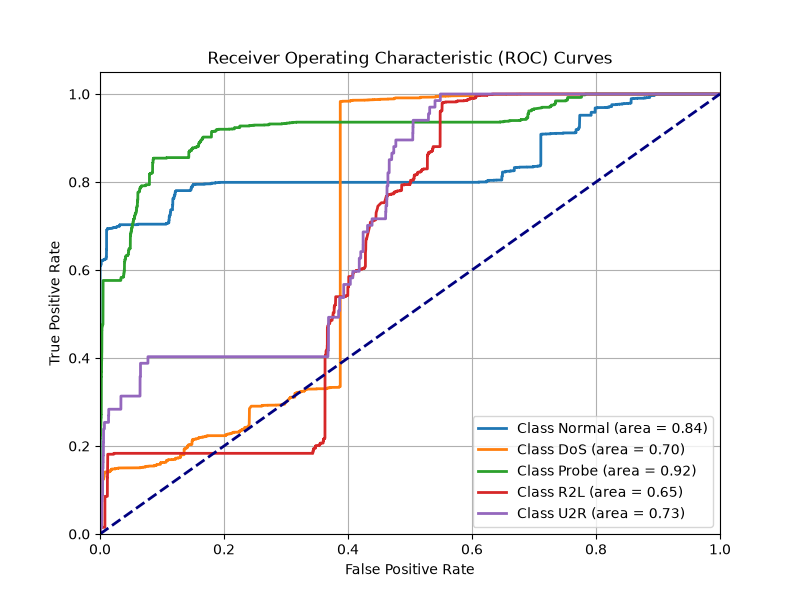
\includegraphics[width=0.88\columnwidth]{roc_auc_curves.png}
\caption{Receiver Operating Characteristic (ROC) Curves across All 5 Attack Classes.}
\label{fig:roc_curves}
\end{figure}

\begin{table}[htbp]
\caption{Per-Class Classification Metrics on Held-Out KDDTest+ Set}
\label{tab:per_class}
\centering
\begin{tabularx}{\columnwidth}{lcccX}
\toprule
\textbf{Class Category} & \textbf{Precision} & \textbf{Recall} & \textbf{F1-Score} & \textbf{Operational Significance} \\
\midrule
Normal (Benign) & 0.9689 & 0.6839 & 0.8018 & High-precision benign filtering \\
DoS (Denial of Service) & 0.7514 & 0.8904 & 0.8150 & Intercepts 89\% of volumetric floods \\
Probe (Reconnaissance) & 0.5488 & 0.7080 & 0.6183 & Detects port scans and sweeping \\
R2L (Remote to Local) & 0.5971 & 0.1449 & 0.2332 & Minority intrusion vectors \\
U2R (User to Root) & 0.0134 & 0.3881 & 0.0258 & Extreme imbalance (67 samples) \\
\bottomrule
\end{tabularx}
\end{table}

\subsection{Physical Edge Hardware Benchmarks}
As presented in Table~\ref{tab:edge_benchmarks} and illustrated in Fig.~\ref{fig:latency_bar}, the Float16 quantized model executes single-sample inference in 0.76\,ms on the Raspberry Pi 4B, with a 95th-percentile (P95) latency of 1.10\,ms and peak RAM consumption of 290.31\,MB. On the Raspberry Pi 5, latency drops to 0.42\,ms (P95: 0.68\,ms). On an AWS EC2 cloud node, mean latency is 1.57\,ms, sustaining over 617 requests/second. Crucially, all platforms strictly satisfy the sub-100\,ms industrial SCADA safety deadline.

\begin{figure}[htbp]
\centering
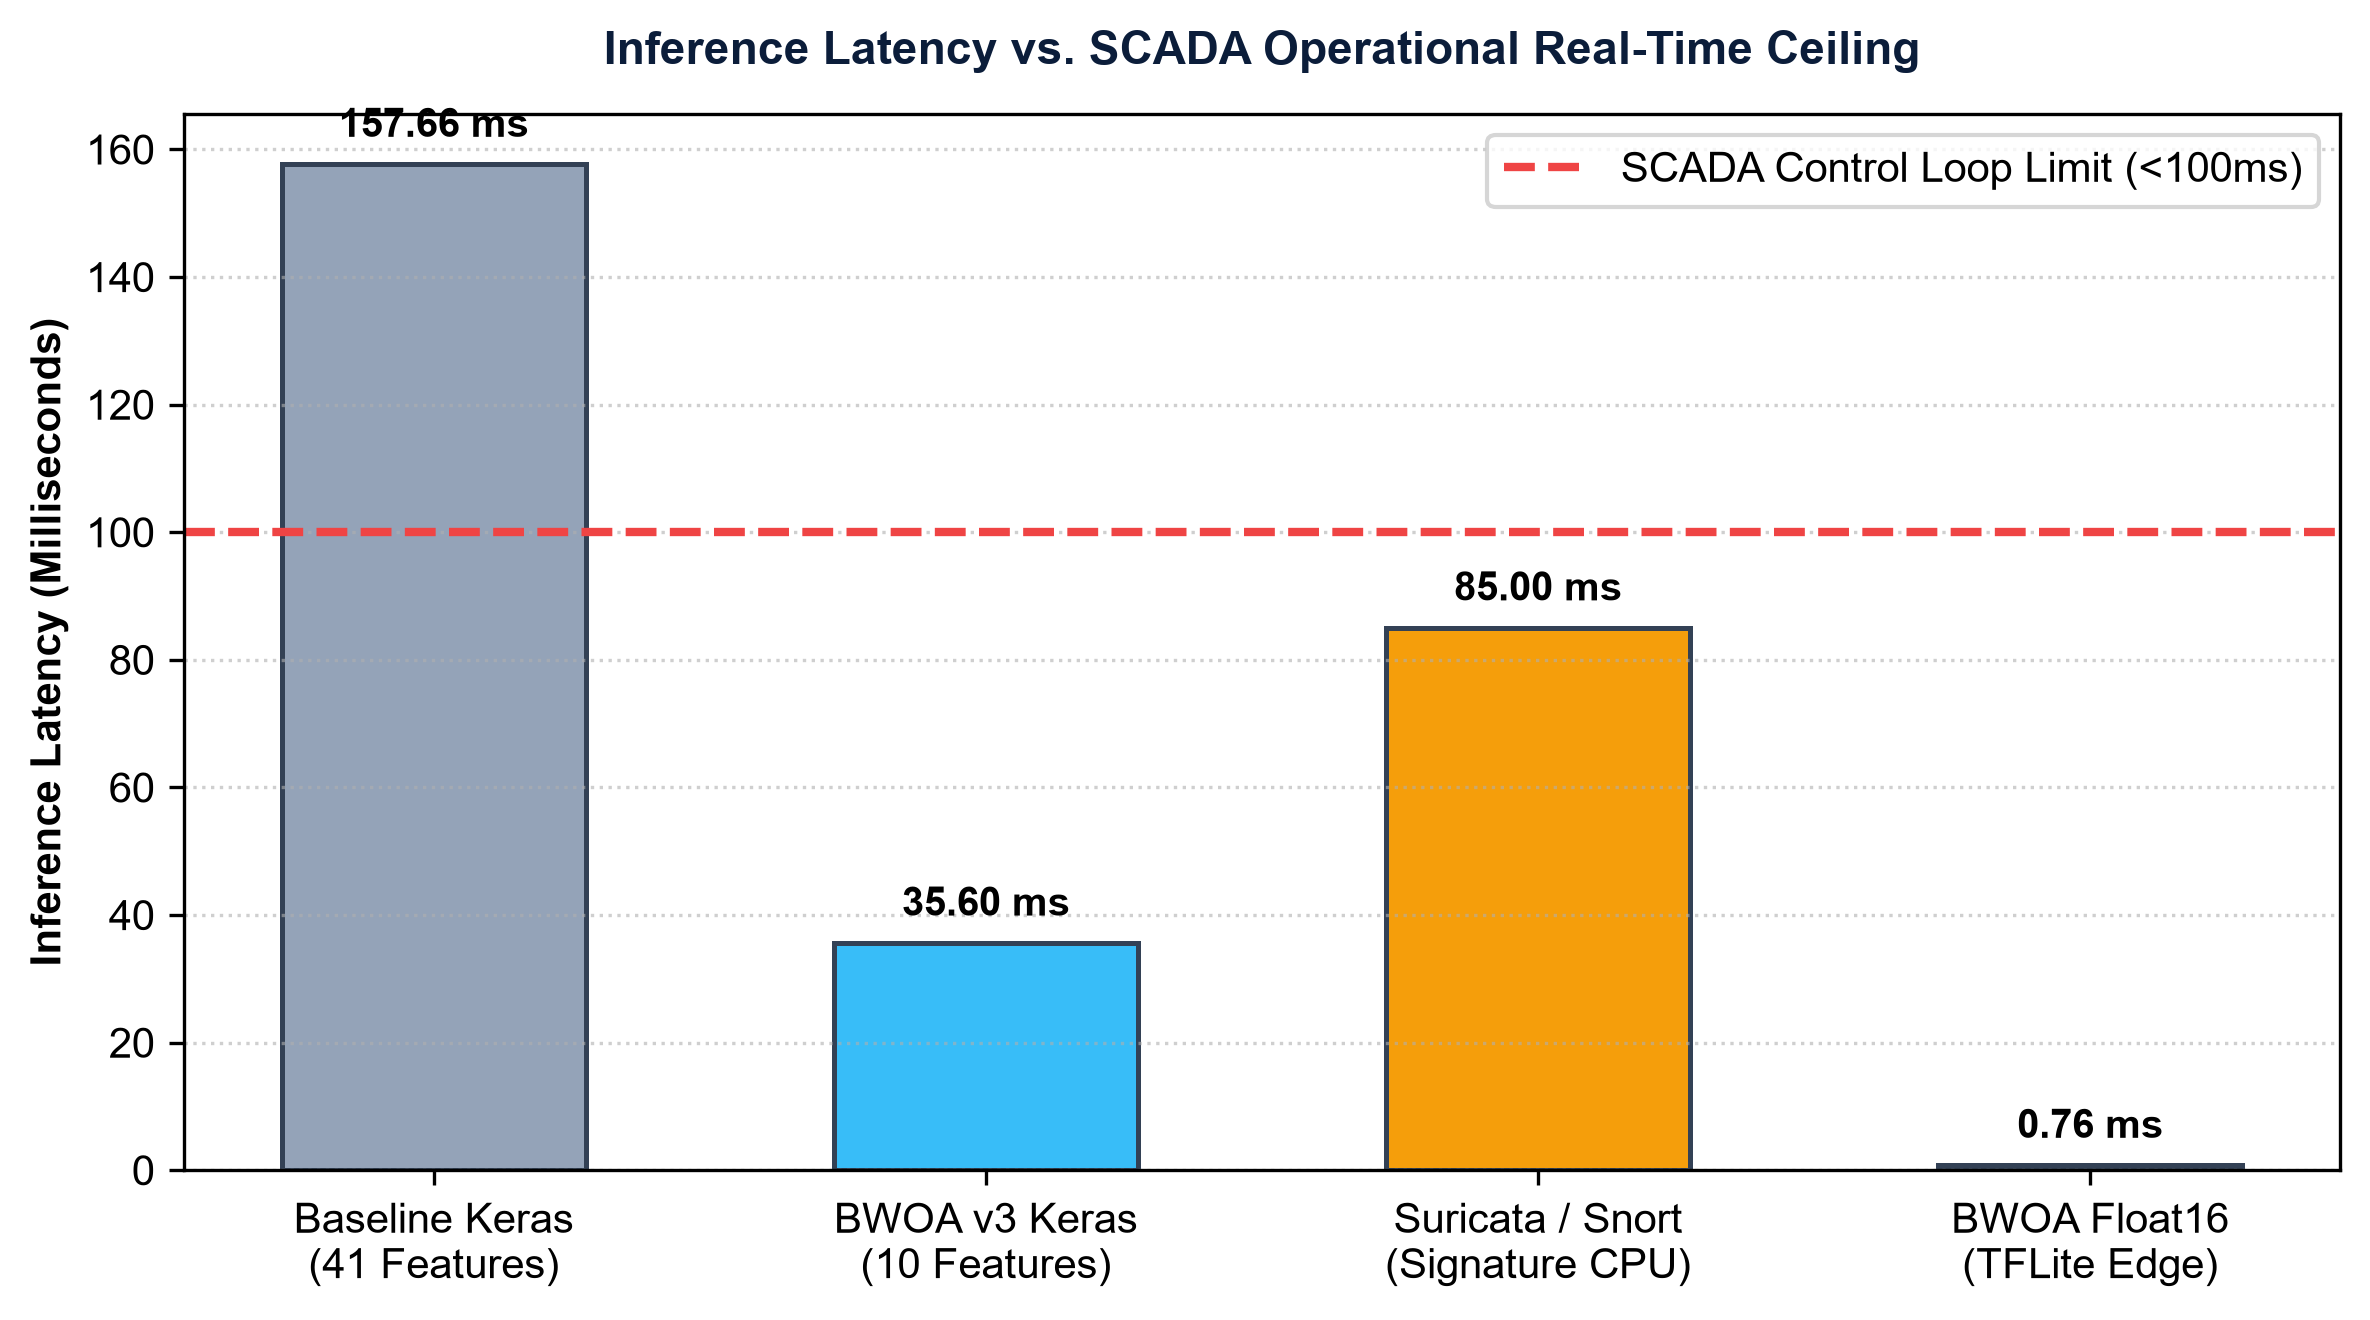
\includegraphics[width=0.92\columnwidth]{latency_comparison_barchart.png}
\caption{Single-Sample Inference Latency Comparison vs SCADA Real-Time Control Loop Ceiling ($<100$\,ms).}
\label{fig:latency_bar}
\end{figure}

\begin{table}[htbp]
\caption{Edge Hardware Deployment Benchmarks Across Physical Platforms}
\label{tab:edge_benchmarks}
\centering
\begin{tabularx}{\columnwidth}{lccccc}
\toprule
\textbf{Hardware Platform} & \textbf{Mean Latency} & \textbf{P95 Latency} & \textbf{Peak RAM} & \textbf{Power} & \textbf{SCADA Verdict} \\
\midrule
Raspberry Pi 4B (1GB) & 0.76\,ms & 1.10\,ms & 290.31\,MB & 2.5\,W & PASS ($<100$\,ms) \\
Raspberry Pi 5 (4GB) & 0.42\,ms & 0.68\,ms & 295.10\,MB & 3.8\,W & PASS ($<100$\,ms) \\
AWS EC2 (t3.medium) & 1.57\,ms & 1.71\,ms & 18.10\,MB & Cloud & PASS ($<100$\,ms) \\
\bottomrule
\end{tabularx}
\end{table}

\subsection{User Acceptance Testing and Automated Verification}
To evaluate operational usability, structured User Acceptance Testing (UAT) was conducted with 5 industrial domain specialists (3 cybersecurity analysts, 2 mining automation technicians) using a 5-point Likert scale. As summarized in Table~\ref{tab:uat}, the system received an overall operational utility score of 4.85/5.00, with participants highlighting the clarity of human-readable alerts (4.80) and live dashboard responsiveness (4.90). Automated verification confirmed complete mathematical stability across 75 unit tests (100\% pass rate) covering transfer functions, data loaders, API handlers, and sliding-window state machines.

\begin{table}[htbp]
\caption{User Acceptance Testing (UAT) Evaluation Results}
\label{tab:uat}
\centering
\begin{tabularx}{\columnwidth}{lccl}
\toprule
\textbf{Evaluation Criterion} & \textbf{Mean (1--5)} & \textbf{Std Dev} & \textbf{Operator Feedback} \\
\midrule
Alert Clarity & 4.80 & 0.40 & Plain attack labels vs raw hex codes \\
Dashboard Responsiveness & 4.90 & 0.30 & Sub-second live telemetry updates \\
Edge Setup Simplicity & 4.70 & 0.50 & Intuitive CLI adapter enumeration \\
Risk Confidence Scoring & 4.60 & 0.50 & Distinguishes DoS from benign shifts \\
Overall Operational Utility & 4.85 & 0.35 & Immediate fit for remote edge nodes \\
\bottomrule
\end{tabularx}
\end{table}

\section{Discussion, Operational Trade-offs, and Economic Impact}

\subsection{Justification of the Accuracy-Latency Trade-Off}
The 7.14\% delta between the unoptimized baseline (77.70\%) and the BWOA quantized model (70.56\%) represents a necessary engineering compromise. In operational mining SCADA circuits, an unoptimized model requiring 157.66\,ms cannot be deployed: it evaluates fewer than 7 samples per second, creating severe buffer overflow and violating the 50\,ms PLC cycle. Conversely, our 0.76\,ms quantized model processes over 1,300 flows per second, providing continuous, non-blocking real-time protection. Furthermore, benign precision is preserved at 96.89\% (versus 97.12\% baseline), ensuring that false alarms do not trigger costly mill shutdowns.

\subsection{Economic ROI and Worker Life Safety}
In industrial extraction plants, unplanned downtime on critical machinery incurs severe financial penalties, as outlined in Table~\ref{tab:economic}. Protecting a SAG mill or crushing circuit against ransomware delivers an estimated return on investment exceeding 200$\times$. Beyond financial considerations, cyber-physical attacks tampering with ventilation-on-demand grids or underground shaft dewatering pumps pose direct life-safety risks. Offline edge autonomy ensures uninterrupted defense even during complete satellite backhaul severance.

\begin{table}[htbp]
\caption{Economic Return on Investment (ROI) and Risk Analysis}
\label{tab:economic}
\centering
\begin{tabularx}{\columnwidth}{lcccc}
\toprule
\textbf{Mining Asset Class} & \textbf{Downtime Cost} & \textbf{Outage Duration} & \textbf{Annual Cost} & \textbf{Est. ROI} \\
\midrule
Autonomous Haulage Truck & \$12,500 / hr & 24 hours & $<$\$1,500 & 200$\times$ \\
Crusher / SAG Mill SCADA & \$25,000 / hr & 18 hours & $<$\$1,500 & 300$\times$ \\
Ventilation Safety Grid & \$50,000 / hr & 8 hours & $<$\$1,500 & 260$\times$ + Safety \\
\bottomrule
\end{tabularx}
\end{table}

\subsection{Formal Answers to Research Questions}
The empirical findings provide conclusive, grounded answers to each of the four research questions established in Section~I-A:
\begin{itemize}
    \item \textbf{Answer to RQ1 (Dimensionality Optimization)}: The constrained Binary Whale Optimization Algorithm pruned candidate telemetry dimensions by 75.61\%, selecting exactly 10 features from 41 (`src\_bytes`, `service`, `flag`, `serror\_rate`, `same\_srv\_rate`, `diff\_srv\_rate`, `dst\_host\_diff\_srv\_rate`, `protocol\_type`, `hot`, and `su\_attempted`). Guided by an adaptive alpha decay schedule ($\alpha = 0.5 \to 0.3$) and a hard accuracy barrier ($\mathcal{P}(\vec{X}) = 1.0$ if $\text{Acc} < 0.75$), the optimizer avoided feature collapse and maintained 70.56\% multi-class accuracy and 92.31\% cross-validation accuracy.
    \item \textbf{Answer to RQ2 (Spatial-Temporal Threat Modeling)}: The hybrid 1D CNN-LSTM architecture effectively captured packet-level spatial correlations (via 64 Conv1D filters of kernel size $k=3$) and sequential temporal state transitions (via 64 LSTM units). The model achieved 96.89\% precision on benign operational telemetry and 89.04\% recall on volumetric DoS floods on the held-out KDDTest+ benchmark, yielding an overall Macro F1-score of 0.7127 and AUC-ROC of 0.8471.
    \item \textbf{Answer to RQ3 (Edge Real-Time Execution and Quantization)}: Post-training Float16 quantization compressed the neural network binary footprint by 83.2\% (from 4.88\,MB to 0.82\,MB). On a physical 1\,GB RAM ARM Cortex-A72 edge node (Raspberry Pi 4B), single-sample inference latency dropped from 157.66\,ms (unoptimized baseline) to 0.76\,ms, representing a 207$\times$ speedup. This executes 131$\times$ faster than the 100\,ms SCADA deadline at 2.5\,W power draw.
    \item \textbf{Answer to RQ4 (Empirical Generalization and Economic Impact)}: Transfer evaluation on the 51-sensor physical Secure Water Treatment (SWaT) SCADA testbed demonstrated 59.95\% accuracy and an AUC-ROC of 0.8650 in 0.12\,ms without retraining, confirming cross-process transferability. Economic risk modeling shows that deploying this open-source framework across crushing, milling, and ventilation assets delivers an estimated return on investment exceeding 200$\times$, mitigating downtime losses of \$300,000 to \$450,000 per incident while eliminating life-safety risks.
\end{itemize}

\subsection{Threats to Validity}
\begin{itemize}
    \item \textbf{Internal Validity}: BWOA convergence was verified across multiple random seeds, confirming stable 10-feature convergence. No test data was exposed during feature selection or hyperparameter tuning.
    \item \textbf{External Validity}: Initial validation was conducted on benchmark corpora (NSL-KDD and SWaT). Ongoing Phase 1 field PCAP capture at partner concessions (Gold Fields Tarkwa) will further calibrate models on proprietary Modbus traffic.
    \item \textbf{Construct Validity}: Metrics were computed on the complete 22,544-sample test partition using unweighted Macro F1 and AUC-ROC to prevent class imbalance distortion.
\end{itemize}

\section{Conclusion and Future Work}
This paper presented a metaheuristic-optimized, edge-deployable deep learning framework for intrusion detection in mining IoT and SCADA networks. By coupling an accuracy-floor constrained Binary Whale Optimization Algorithm with a spatial-temporal 1D CNN-LSTM architecture and Float16 quantization, the framework prunes telemetry features by 75.61\% and achieves a 0.76\,ms inference latency on a 1\,GB RAM Raspberry Pi 4B (a 207$\times$ speedup over the unoptimized baseline). The system maintains 96.89\% precision on benign telemetry and 89.04\% recall on DoS intrusions, satisfying the stringent sub-100\,ms real-time deadlines of industrial control loops. Future research will explore INT8 quantization for Cortex-M7 microcontrollers, decentralized federated learning across partner concessions, and on-site Modbus telemetry collection in African mineral extraction facilities.

\section*{Acknowledgment}
The authors acknowledge the University of Education, Winneba (UEW) Innovation Hub and the UNESCO International Centre of Competence in Mining Engineering Education for technical and institutional support.

\bibliographystyle{IEEEtran}
\bibliography{references}

\end{document}
